%%%%%%%%%%%%%%%%%%%%%%%%%%%%%%%%%%%%%%%%%
% Journal Article
% LaTeX Template
% Version 1.4 (15/5/16)
%
% This template has been downloaded from:
% http://www.LaTeXTemplates.com
%
% Original author:
% Frits Wenneker (http://www.howtotex.com) with extensive modifications by
% Vel (vel@LaTeXTemplates.com)
%
% License:
% CC BY-NC-SA 3.0 (http://creativecommons.org/licenses/by-nc-sa/3.0/)
%
%%%%%%%%%%%%%%%%%%%%%%%%%%%%%%%%%%%%%%%%%

%----------------------------------------------------------------------------------------
%	PACKAGES AND OTHER DOCUMENT CONFIGURATIONS
%----------------------------------------------------------------------------------------

\documentclass[twoside,twocolumn]{article}

%\usepackage{booktabs,caption}
\usepackage[flushleft]{threeparttable}
\usepackage{graphicx}
\usepackage{blindtext} % Package to generate dummy text throughout this template 

\usepackage[sc]{mathpazo} % Use the Palatino font
\usepackage[T1]{fontenc} % Use 8-bit encoding that has 256 glyphs
\linespread{1.05} % Line spacing - Palatino needs more space between lines
\usepackage{microtype} % Slightly tweak font spacing for aesthetics

\usepackage[english]{babel} % Language hyphenation and typographical rules

\usepackage[hmarginratio=1:1,top=32mm,columnsep=20pt, left= 2.35cm, right = 2.35cm]{geometry} % Document margins
\usepackage[hang, small,labelfont=bf,up,textfont=it,up]{caption} % Custom captions under/above floats in tables or figures
\usepackage{booktabs} % Horizontal rules in tables

\usepackage{lettrine} % The lettrine is the first enlarged letter at the beginning of the text

\usepackage{enumitem} % Customized lists
\setlist[itemize]{noitemsep} % Make itemize lists more compact

\usepackage{abstract} % Allows abstract customization
\renewcommand{\abstractnamefont}{\normalfont\bfseries} % Set the "Abstract" text to bold
\renewcommand{\abstracttextfont}{\normalfont\small\itshape} % Set the abstract itself to small italic text

\usepackage{titlesec} % Allows customization of titles
\renewcommand\thesection{\Roman{section}} % Roman numerals for the sections
\renewcommand\thesubsection{\roman{subsection}} % roman numerals for subsections
\titleformat{\section}[block]{\large\scshape\centering}{\thesection.}{1em}{} % Change the look of the section titles
\titleformat{\subsection}[block]{\large}{\thesubsection.}{1em}{} % Change the look of the section titles

\usepackage{fancyhdr} % Headers and footers
\pagestyle{fancy} % All pages have headers and footers
\fancyhead{} % Blank out the default header
\fancyfoot{} % Blank out the default footer
%\fancyhead[C]{Running title $\bullet$ May 2016 $\bullet$ Vol. XXI, No. 1} % Custom header text
\fancyfoot[RO,RE]{\thepage} % Custom footer text

\usepackage{titling} % Customizing the title section

\usepackage{hyperref} % For hyperlinks in the PDF

%----------------------------------------------------------------------------------------
%	TITLE SECTION
%----------------------------------------------------------------------------------------

\setlength{\droptitle}{-4\baselineskip} % Move the title up

\pretitle{\begin{center}\huge\bfseries} % Article title formatting
\posttitle{\end{center}} % Article title closing formatting
\title{Nummerical Integration Using Gaussian Quadrature and Monte Carlo Method } % Article title

\author{%
\textsc{Andreas Fagerheim}\thanks{\url{https://github.com/AndreasFagerheim/Fys4150}} \\[1ex] % Your name
\normalsize Department of Physics, University of Oslo, Norway \\ % Your institution
%\normalsize \href{mailto:john@smith.com}{john@smith.com} % Your email address
%\and % Uncomment if 2 authors are required, duplicate these 4 lines if more
%\textsc{Jane Smith}\thanks{Corresponding author} \\[1ex] % Second author's name
%\normalsize University of Utah \\ % Second author's institution
%\normalsize \href{mailto:jane@smith.com}{jane@smith.com} % Second author's email address
}
\date{\today} % Leave empty to omit a date

%---------------------------------------------------------------------------------------
\renewcommand{\maketitlehookd}{%
\begin{abstract}

This article set forth to integrate a six-dimensional integral which is 
used to determine the ground state
correlation energy between two electrons in a helium atom.  The
integral appears in many quantum mechanical applications. We will first solve the integral true a brute force manner and employ both Gauss-Legendre and
Gauss-Laguerre quadrature and Monte-Carlo integration. 


\end{abstract}
}

%----------------------------------------------------------------------------------------

\begin{document}

% Print the title
\maketitle

%----------------------------------------------------------------------------------------
%	ARTICLE CONTENTS
%----------------------------------------------------------------------------------------
\section{Introduction}
\section{Theory}

%\lettrine[nindent=0em,lines=3]{W} 
The wave function of each electron can be assumed to be modelled like
the single-particle wave function of an electron in the hydrogen
atom. The single-particle wave function for an electron $i$ in the
$1s$ state can the be modelled by:



\begin{equation}
		\psi_{1s}({\bf r}_i)  =   e^{-\alpha r_i}.
\end{equation}
The parameter $\alpha$ is connected to the charge of the atom and will in our case be set to equal 2 to correspond to the helium atom $Z = 2$. Furthermore $r_i$ is the magnitude of the position vector ${\bf r}_i$ and is given by
\[
r_i = \sqrt{x_i^2+y_i^2+z_i^2}.
\]
and
\[
   {\bf r}_i =  x_i {\bf e}_x + y_i {\bf e}_y +z_i {\bf e}_z ,
\]
The ansatz for the wave function for two electrons is then given by the product of two 
so-called 
$1s$ wave functions as 
\[
   \Psi({\bf r}_1,{\bf r}_2)  =   e^{-\alpha (r_1+r_2)}.
\]

Note that it is not possible to find a closed-form or analytical
solution to Schr\"odinger's equation for two interacting electrons in
the helium atom.

The integral we need to solve is the quantum mechanical expectation
value of the correlation energy between two electrons which repel each
other via the classical Coulomb interaction, namely

\begin{equation} \label{integral}
   \langle \frac{1}{|{\bf r}_1-{\bf r}_2|} \rangle=\int_{-\infty}^{\infty} d{\bf r}_1d{\bf r}_2  e^{-2\alpha (r_1+r_2)}\frac{1}{|{\bf r}_1-{\bf r}_2|}.
\end{equation}

Note that our wave function is not normalized, but we dont nedd to worry abou this.

This integral can be solved in closed form and the answer is
$5\pi^2/16^2$.

%------------------------------------------------

\section{Methods}
The integral will be solved using four numerical methods. First numerical integration method  we set forth to explore is the Gaussian Quadrature which concept is to make use of a weight function $W(x)$ to give more emphasis to one part of the interval we integrate over than another. The basic idea behind this method is to approximate the integral
\begin{equation}ß
   I = \int_{a}^{b}f(x)dx = \int_{a}^{b} W(x)g(x) dx \approx\sum_{i=1}^{N} w_ig(x_i)
\end{equation}
Where $w_i$ is the weights and obtained through orthogonal polynomials. These polynomials are orthogonal in some interval $[a,b]$ and the points $x_i$ is constrained to lie in this interval. Different weight functions, $W(x)$ gives rise to different methods and we will look  closer at Gaussian-Legendre ($W(x) = 1$) and Gaussian-Laguerre ($W(x)  = x^\alpha e^{-x}$). These weight functions get their polynomials from the intervals $[-1,1]$ and $[0,\infty\rangle$. The integral (\ref{integral})
we are working to solve has the limits $x\in[-\infty,\infty]$ and therefore need to rewrite the integral for to be in the right limits. By changing variable
\begin{equation}
		t= \frac{b-a}{2}x + \frac{b+a}{2}
\end{equation}
we can do this
\begin{equation}
		\int_a^b f(x) dx = \frac{b-a}{2} \int_{-1}^1f( \frac{b-a}{2}x + \frac{b+a}{2})
\end{equation}


\subsection{Gauss-Legendre Quadrature}
The weight function $W(x) = 1$ is used in Gauss-Legendre Quadrature and use Legendre polynomials in the interval $[-1,1]$

\begin{figure}[h]
\center
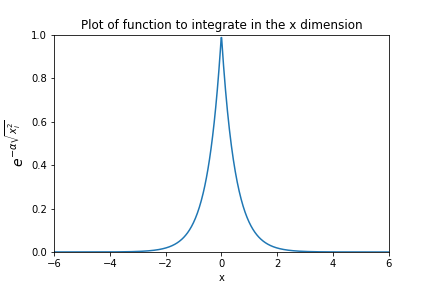
\includegraphics[scale=0.55]{figure1.png}
\caption{Plot of the single particle wave function to find appropiate limits}
\end{figure}
\subsection{Gauss-Laguerre Quadrature}

\begin{equation}
	\tilde{x}_i = tan(\frac{\pi}{4}(1+x_i)
\end{equation}

\begin{equation}
	\tilde{w}_i = \frac{\pi}{4}\frac{w_i}{\cos^2(\frac{\pi}{4}(1+x_i))}
\end{equation}

where $w_i$ and$x_i$ are the original weights and mesh points in the interval [-1,1], while $tilde{w}_i$ and $\tilde{x}_i$ are the new weights and mesh points in the interval $[0,\infty\rangle$.
\subsection{Monte Carlo brute force}
\subsection{Monte Carlo method improved}

Text requiring further explanation\footnote{Example footnote}.

%------------------------------------------------

\section{Results}


\subsection{Gauss-Legendre Quadrature}
The implemented Gauss-Legendre Quadrature method yields the results given in \textbf{Table 1} when used to solve (\ref{integral}). With $N=25$ the relative error is at its lowest, but is still $1.9 \%$.


\par
\begin{table}[h]

\begin{center}
\begin{threeparttable}
\begin{tabular}{|l|l|c|}
\hline
N  & Integral & \multicolumn{1}{l|}{Relative error} \\ \hline
5  & 0.354602 & 0.83950         \\ \hline
10 & 0.129834 & 0.32650         \\ \hline
15 & 0.199475 & 0.03480         \\ \hline
20 & 0.177065 & 0.08145        \\ \hline
25 & 0.18911  & 0.01897        \\ \hline
30 & 0.185796 & 0.03616        \\ \hline
\end{tabular}
%\begin{tablenotes}
%\item[1] qwerty; \item[2] asdfgh
%\end{tablenotes}
\end{threeparttable}
\end{center}
\label{table:tableLegendre}
\caption{Results from using Gauss-Legendre Quadrature for calculating the integral with an exact solution equal to $0.192766$}
\end{table}


%------------------------------------------------

\section{Discussion}

\subsection{Subsection One}

A statement requiring citation \cite{Figueredo:2009dg}.
\blindtext % Dummy text

\subsection{Subsection Two}

\blindtext % Dummy text

%----------------------------------------------------------------------------------------
%	REFERENCE LIST
%----------------------------------------------------------------------------------------

\begin{thebibliography}{99} % Bibliography - this is intentionally simple in this template

\bibitem[Figueredo and Wolf, 2009]{Figueredo:2009dg}
Figueredo, A.~J. and Wolf, P. S.~A. (2009).
\newblock Assortative pairing and life history strategy - a cross-cultural
  study.
\newblock {\em Human Nature}, 20:317--330.
 
\end{thebibliography}

%----------------------------------------------------------------------------------------

\end{document}